%  For slides only
%%% Usage:
%% $ cat slidesonly.tex unitXX-foo.tex | pdflatex
%% $ pdfjam -o unitXX-slides{a/b/...}.pdf texput.pdf '1,{1stpage}-{lastpage}'

\documentclass{beamer} 
\newcommand{\tcw}{\textcolor{black}}
\newcommand{\mynoteonly}{}
\newcommand{\nottheirhandout}{handout:0}

% % For handout
%%% Usage:
%% $ cat handout.tex unitXX-foo.tex | pdflatex
%% $ pdfjam -o unitXX-handout{a/b/...}.pdf texput.pdf '{1stpage}-{lastpage}'
\documentclass[handout]{beamer}
\usepackage{pgfpages}
\pgfpagesuselayout{4 on 1}[letterpaper,border shrink=5mm]%\nofiles

\mode<handout>{\setbeamercolor{background canvas}{bg=black!5}}
\newcommand{\tcw}{\textcolor{structure.bg}}
\newcommand{\mynoteonly}{| handout:0}
\newcommand{\nottheirhandout}{handout:0}

%For handout + mynotes
%% Usage:
%% $ cat handout+mynotes.tex unitXX-foo.tex | pdflatex
%% $ pdfjam --nup 1x4 -o unitXX-foo-wmn{a/b/...}.pdf texput.pdf '1,{1stpage}-{lastpage}'
\documentclass[handout]{beamer}
\usepackage{pgfpages}
%%\pgfpagesuselayout{2 on 1}[letterpaper,border shrink=5mm] 
\setbeameroption{show notes on second screen=left}
\newcommand{\tcw}{\textcolor{black}}
\newcommand{\mynoteonly}{}
\newcommand{\nottheirhandout}{}

\newcommand{\igrphx}[2][width=\linewidth]{\includegraphics[#1]{images/#2}}

\renewcommand{\strut}{\rule{0pt}{3ex}}

% Frame note commands, with time budget updating
\newcounter{timeTotal}
\newcommand{\printUpdateTimeTotal}[1]{ \addtocounter{timeTotal}{#1}
  \textrm{(#1 min budgeted)} \hfill \textbf{Finish by
    \arabic{timeTotal}\ min from start}\\[1ex]}
\newcommand{\tnote}[3][10]{#2 \note{#2: #3 \\[.5ex]} \printUpdateTimeTotal{#1}}
\newcommand{\itnote}[2][10]{\note{ \begin{itemize} #2 \end{itemize}
\vfill \noindent  \printUpdateTimeTotal{#1} }}
\newcommand{\ennote}[2][10]{\note{ \begin{enumerate} #2 \end{enumerate}
\vfill \noindent  \printUpdateTimeTotal{#1} }}
\newcommand{\Note}[2][10]{\note{ #2 \mbox{ }\\ \vfill \noindent  \printUpdateTimeTotal{#1} }}

\newenvironment{Column}[1][.5\linewidth]{\begin{column}{#1}}{\end{column}}

\mode<handout>{\beamertemplatesolidbackgroundcolor{black!5}} 
\mode<article>{\usepackage{fullpage}}
\mode<presentation>
{
  \usetheme{Boadilla}
  % or ...

  \setbeamercovered{transparent}
  % or whatever (possibly just delete it)
}
\usepackage{url}
\usepackage{ulem}

\usepackage[english]{babel}
% or whatever

\usepackage[latin1]{inputenc}
% or whatever

\usepackage{times}
\usepackage[T1]{fontenc}
% Or whatever. Note that the encoding and the font should match. If T1
% does not look nice, try deleting the line with the fontenc.

\AtBeginSubsection[]
{
  \begin{frame}<beamer>
    \frametitle{Outline}
    \tableofcontents[subsectionstyle=show/shaded/hide]
  \end{frame}
}

\AtBeginSection[]
{
  \begin{frame}<beamer>
    \frametitle{Outline}
    \tableofcontents[hideothersubsections,sectionstyle=show/shaded]
  \end{frame}
}


% If you wish to uncover everything in a step-wise fashion, uncomment
% the following command: 

%\beamerdefaultoverlayspecification{<+->}

%USEFUL CODE TEMPLATES:
%\begin{itemize}[<+-| alert@+>]


% \begin{frame}[fragile]


% \begin{columns}
% \column{.4\textwidth}  
%   \begin{itemize}
%   \item<1-| alert@1> Why sample twice?
%   \item<2-| alert@2> Illustrative example.
%   \item<3-| alert@3> PSU's and SSU's.
%   \item<4-| alert@4> Stratification in combination with two-stage cluster sampling.
%   \item<5-| alert@5> Detailed example.
%   \end{itemize}
% \column{.6\textwidth}
% \only<2| handout:0>{
% \includegraphics[width=\textwidth]{nursingHomes}}
% \only<5| handout:1>{
% \includegraphics[width=\textwidth]{hosp_cover}}
% \end{columns}

% FOR INCLUDING R CODE. 
%\usepackage{listings}
%\lstset{language=R}
% \begin{frame}[fragile]
% \frametitle{Some code}
% \begin{lstlisting}
% > plot(myobj)
% > rm(myobj)
% \end{lstlisting}  
% \end{frame}

%\addtocounter{framenumber}{-1}


\usepackage{amsmath,amsthm}
\usepackage{wasysym,pifont}
\usepackage{Sweave}
\usepackage{ulem}
\usepackage{textcomp}
\usepackage{versions}
%% amsthm-type theorem environment specifications -- 
%% see amsthdoc.pdf in amscls documentation
\theoremstyle{plain}
\newtheorem{prop}{Proposition}[section]
\newtheorem{lem}[prop]{Lemma}

\newtheorem*{thm}{Proposition}
\newtheorem*{cor}{Corollary}

\theoremstyle{definition}
\newtheorem{defn}{Definition}[section]

\newcommand{\Pdistsym}{P}
\newcommand{\Pdistsymn}{P_n}
\newcommand{\Qdistsym}{Q}
\newcommand{\Qdistsymn}{Q_n}
\newcommand{\Qdistsymni}{Q_{n_i}}
\newcommand{\Qdistsymt}{Q[t]}
\newcommand{\dQdP}{\ensuremath{\frac{dQ}{dP}}}
\newcommand{\dQdPn}{\ensuremath{\frac{dQ_{n}}{dP_{n}}}}
\newcommand{\EE}{\ensuremath{\mathbf{E}}}
\newcommand{\EEp}{\ensuremath{\mathbf{E}_{P}}}
\newcommand{\EEpn}{\ensuremath{\mathbf{E}_{P_{n}}}}
\newcommand{\EEq}{\ensuremath{\mathbf{E}_{Q}}}
\newcommand{\EEqn}{\ensuremath{\mathbf{E}_{Q_{n}}}}
\newcommand{\EEqni}{\ensuremath{\mathbf{E}_{Q_{n[i]}}}}
\newcommand{\EEqt}{\ensuremath{\mathbf{E}_{Q[t]}}}
\newcommand{\PP}{\ensuremath{\mathbf{Pr}}}
\newcommand{\PPp}{\ensuremath{\mathbf{Pr}_{P}}}
\newcommand{\PPpn}{\ensuremath{\mathbf{Pr}_{P_{n}}}}
\newcommand{\PPq}{\ensuremath{\mathbf{Pr}_{Q}}}
\newcommand{\PPqn}{\ensuremath{\mathbf{Pr}_{Q_{n}}}}
\newcommand{\PPqt}{\ensuremath{\mathbf{Pr}_{Q[t]}}}
\newcommand{\var}{\ensuremath{\mathbf{V}}}
\newcommand{\varp}{\ensuremath{\mathbf{V}_{P}}}
\newcommand{\varpn}{\ensuremath{\mathbf{V}_{P_{n}}}}
\newcommand{\varq}{\ensuremath{\mathbf{V}_{Q}}}
\newcommand{\cov}{\ensuremath{\mathbf{Cov}}}
\newcommand{\covp}{\ensuremath{\mathbf{Cov}_{P}}}
\newcommand{\covpn}{\ensuremath{\mathbf{Cov}_{P_{n}}}}
\newcommand{\covq}{\ensuremath{\mathbf{Cov}_{Q}}}

\newcommand{\hatvar}{\ensuremath{\widehat{\mathrm{Var}}}}
\newcommand{\hatcov}{\ensuremath{\widehat{\mathrm{Cov}}}}

\newcommand{\sehat}{\ensuremath{\widehat{\mathrm{se}}}}

\newcommand{\combdiff}[1]{\ensuremath{\Delta_{{z}}[#1]}}
\newcommand{\Combdiff}[1]{\ensuremath{\Delta_{{Z}}[#1]}}

\newcommand{\psvec}{\ensuremath{\varphi}}
\newcommand{\psvecgc}{\ensuremath{\tilde{\varphi}}}


\newcommand{\atob}[2]{\ensuremath{#1\!\! :\!\! #2}}
\newcommand{\stratA}{\ensuremath{\mathbf{S}}}
\newcommand{\stratAnumstrat}{\ensuremath{S}}
\newcommand{\sAsi}{\ensuremath{s}}

\newcommand{\permsd}{\ensuremath{\sigma_{\Pdistsym}}}
% \newcommand{\dz}[1]{\ensuremath{d_{z}[{#1}]}}
\newcommand{\dZ}[1]{\ensuremath{d_{Z}[{#1}]}}
\newcommand{\tz}[1]{\ensuremath{t_{{z}}[#1]}}
\newcommand{\tZ}[1]{\ensuremath{t_{{Z}}[#1]}}


\newlength{\tabcolsepadj}
\setlength{\tabcolsepadj}{1.3mm}

%%% NEWBLOCK UNDEFINED BUG
\def\newblock{\hskip .11em plus .33em minus .07em}

%%% tightlist undefined control sequence bug 
%%% http://tex.stackexchange.com/questions/257418/error-tightlist-converting-md-file-into-pdf-using-pandoc
\providecommand{\tightlist}{%
  \setlength{\itemsep}{0pt}\setlength{\parskip}{0pt}}
\newcommand{\igrphx}[2][width=\linewidth]{\includegraphics[#1]{images/#2}}

\renewcommand{\strut}{\rule{0pt}{3ex}}

\newenvironment{Column}[1][.5\linewidth]{\begin{column}{#1}}{\end{column}}

\usepackage{tikz}
\usepackage{tikz-cd}
\usepackage{textpos}

\usetikzlibrary{arrows} % also see \tikzstyle spec below after \begin{doc}

\newcommand{\mlpnode}[1]{\tikz[baseline=-.5ex] \coordinate (#1) {};}
%\newcommand{\mlpnode}[1]{\raisebox{.5ex}{\pnode{#1}}}


\usepackage{xspace}

\includeversion{pedantic} % \excludeversion
\tikzstyle{every picture}+=[remember picture]


% copied from CSCAR svn repo, `dissdefs.tex`
%\usepackage{xspace}
\newcommand{\satm}{\mbox{\textsc{sat-m}}\xspace}
\newcommand{\satv}{\mbox{\textsc{sat-v}}\xspace}
\newcommand{\upm}{\mbox{\textsc{urm}}\xspace}
\newcommand{\asian}{\mbox{\textsc{asian}}\xspace}
\newcommand{\presatm}{\mbox{\textsc{pre-m}}\xspace}
\newcommand{\premath}{\mbox{\textsc{pre-m}}\xspace}
\newcommand{\presatv}{\mbox{\textsc{pre-v}}\xspace}
\newcommand{\preverb}{\mbox{\textsc{pre-v}}\xspace}
\newcommand{\parentsinc}{\mbox{\textsc{incm}}\xspace}
\newcommand{\gpa}{\mbox{\textsc{gpa}}\xspace}
\newcommand{\dadsed}{\mbox{\textsc{dadsed}}\xspace}
\newcommand{\momsed}{\mbox{\textsc{momsed}}\xspace}
\newcommand{\avgeng}{\mbox{\textsc{e-gpa}}\xspace}
\newcommand{\avgmath}{\mbox{\textsc{m-gpa}}\xspace}
\newcommand{\avgnatsci}{\mbox{\textsc{ns-gpa}}\xspace}
\newcommand{\avgssci}{\mbox{\textsc{ss-gpa}}\xspace}
\newcommand{\coach}{\mbox{\textsc{coach}}\xspace}
\newcommand{\dadcoll}{\mbox{\textsc{dadcoll}}\xspace}
\newcommand{\aavg}{\mbox{\textsc{a-avg}}\xspace}

\newcommand{\teeW}{\ensuremath{t_{W}}}
\newcommand{\pcor}{\ensuremath{\rho_{y \cdot w|z\mathbf{x}}}}





\date{ICPSR Session 2 (July 19, 2021)}


\title{Unit 2: Estimation in experiments}
% \author moved to beamer-preamble-*-all.tex

\begin{document}


% putting `\begin{frame}`/ `\end{frame}` in announcement-of-the-day.tex lets us 
% put frame notes into that file
% announcement-of-the-day.tex not part of repo
%\InputIfFileExists{announcement-of-the-day.tex}{% from https://tex.stackexchange.com/questions/100663/if-the-remote-file-exists-then-include-it-else-include-the-local-one
  % File personal/bar.tex exists and is read
  \input{announcement-of-the-day}
%}{%
  % File personal/bar.tex is not found, try bar.tex
%}




\begin{frame}<\nottheirhandout>{Overview of Unit 2, estimating causal parameters}
  \begin{itemize}
  \item In coffee/tea tasting examples, easier to think about whether causation occurred than how one might measure it.
  \item Now, examples that lend themselves to talk of ``average causal effects,'' etc.
%  \item ``effect'' will have a different and more specific meaning than elsewhere in statistics; we'll begin by talking about it.
  \item We'll continue to use methods that don't care whether outcomes
    are binary, continuous, etc, and avoid distributional assumptions.
  \item  First example of a  twist of the study design that the
    analysis has to take into account (clustering).   
  \item We'll add an assumption of \textit{non-interference} (aka ``SUTVA'')
  \item In contrast to unit 1, focus on estimation rather than testing.
  \end{itemize}
\end{frame}


\section{Experiment design \& probability notation} 


\begin{frame}{Common design aspects of randomized studies} 
  \begin{itemize}
  \item<1-> Common properties of small, simple experiments:
    \begin{itemize}
    \item balanced 
    \item complete (e.g., assignment by \texttt{sample()} or by card shuffle)
    \item simple (e.g., card shuffle \textit{or} coin toss)
    \end{itemize}
  \item<2-> Common complications:
    \begin{itemize}
    \item<2-> pairs
    \item<2-> blocks
    \item<2-> cluster-level assignment
    \end{itemize}
  \item<3-> We'll handle complications by simplification, reorganizing so that we're looking at 1 or more simpler studies.
  \item<4-> (Same considerations will apply to non-randomized studies.)
  \end{itemize}

\end{frame}
\note{Examples:
  \begin{itemize}
  \item Fisher/coffee tasting
  \item variations of the tasting experiment envisioned by us, by Neyman
  \item Gosnell, \ldots, Arcenaux GOTV
  \end{itemize}
}


\begin{frame}<1>[label=EEreviewFr]{Review: expected value\footnote{See also G\& G, ch 2}}

  \begin{itemize}
  \item Consider arbitrary \textit{random variables} $V$, $W$.
  \item (For simplicity, assume discrete --- as $\mathbf{Z}$ generally is.)
  \item  $\EE(V) = \sum_{\mbox{all v's}} v\mathrm{P}(V=v) $.
  \item<2-> For constant $\alpha$, $\EE  \alpha = \alpha$
  \item<2-> For constants $\alpha, \beta$, $\EE (\alpha + \beta V) =
    \alpha + \beta\EE(V)$.
  \item<2-> Also $\EE(\alpha V + \beta W) = \alpha \EE(V) + \beta \EE(W)$. 
  \item<3-> In particular, 
$$\EE\left(\frac{1}{n} \sum_{i=1}^n V_i\right) = \frac{1}{n}
\sum_{i=1}^n \EE V_i.$$
  \end{itemize}


\end{frame}
\note{  Note to self: Calculus of expectation items saved for later}

\begin{frame}<\nottheirhandout>{Exercise: random assignment methods}
{\footnotesize (based on G\&G ch1 ex 5)}

\begin{enumerate} \addtocounter{enumi}{8}
\item

A researcher plans to ask six subjects to donate time to an adult
literacy program. Each subject will be asked to donate either 30
($Z=0$) or 60 ($Z=1$)
minutes. The researcher is considering three methods for randomizing
the treatment. Method I is to make independent decisions for each
subject, tossing a coin each time. Method C is to
write ``30'' and ``60'' on three playing cards each, and then shuffle
the six cards. Method P tosses one coin for each of the 3 pairs
$(1,2)$, $(3,4)$, $(5,6)$, asking for 30 (60) minutes from exactly one
member of each pair. 
  
\begin{itemize}
\item[a] Discuss strengths \& weaknesses of each method.
\item[b] How would your answers to (a) change if $n: 6 \mapsto 600$?
\item[c] Determine $\mathrm{E}\left[  Z_{1} \right]$  under each method.
\item[d] Determine $\mathrm{E} \left[  Z_{1} + Z_{2} + \cdots + Z_{6} \right]$ under each method.
\end{itemize}

\end{enumerate}

\end{frame}

\againframe<2\mynoteonly>{EEreviewFr}




\begin{frame}{Notational conventions for random variables \& vectors}
  
  \begin{itemize}
\item Matrices \& vectors: $(a_{1}, a_{2}, \ldots, a_{n})' = \left(
    \begin{array}{c}
      a_{1} \\ \vdots \\ a_{n}
    \end{array}
\right)$ ;  $\left(
      \begin{array}{c}
        b_{1} \\  \vdots \\ b_{n}\\
      \end{array}
\right)' = (b_{1}, \ldots, b_{n})$.
  \item By convention, $X, Y, Z$ denote random variables (RVs); $x, y, z$, realizations of the RVs.
    \begin{itemize}
    \item Rosenbaum (a statistician) observes this convention\ldots
    \item as I will.
    \item G\& G (political scientists) appear not to.
    \end{itemize}
 \item $x_{i}$= subject $i$ measurement; $\mathbf{x} =(x_{1}, \ldots, x_{n})'$ column of measurements
  \item $Z_i$= random variable for subject $i$; $\mathbf{Z}=(Z_1, Z_2,
    \ldots, Z_n)'$ (a ``random vector'').  
  \item So $\mathbf{z}=(z_1, z_2, \ldots, z_n)'$ denotes a particular
    realization of $\mathbf{Z} $.
  \item Vector cross products: $\mathbf{a}'\mathbf{b}  = a_{1}b_{1} + \cdots + a_{n}b_{n}$
  \end{itemize}


\end{frame}

\begin{frame}<\nottheirhandout>{Exercise: random assignment methods}
{\footnotesize (G\&G ch1 ex 5)}

\begin{enumerate} \addtocounter{enumi}{9}
\item 
{\small \input{assignments/gg15ii}
}
\end{enumerate}
\vfill

% \visible<2>{Either way, canonical analyses treat observations as
% \textit{independent} samples, sizes $n_{0}$ and $n_{1}$, from
% ``\textit{superpopulations}'' of size $N_{0}, N_{1} \approx
% \infty$.  We'll see how one such analysis flows from more serious assumptions.}
\end{frame}


\section{Potential outcome schedules}

\begin{frame}{Four study examples} 


\begin{columns}
\begin{Column}
1. An election campaign randomized (complete) at the precinct level, w/ varying
levels of ``compliance.''\\[2ex]
 2. A quasi-experiment: Hospital admissions on Friday the 13ths vs
Friday the 6ths.\\
{\small
\begin{tabular}{ll|rr} \hline
Yr & Month &	6th &	13th \\ \hline
89 & Oct. &	9 &	13 \\
90 & July &	6 &	12 \\
91 & Sep. &11 &	14 \\
91 & Dec. &	11 &	10 \\
92 & Mar. &	3 &	4 \\
92 & Nov. &	5 &	12 \\ \hline
\end{tabular}
}
\end{Column}
\begin{Column}

3. A natural experiment (w/ simple randomization)%
%\footnote{Example from Gerber and Green (2012)  ch. 2.}
:
\\
        \igrphx{ggch2tab2}\\[2ex]

4. Fisher's tea-tasting experiment. 

\end{Column}
\end{columns}

  
\end{frame}


\begin{frame}{Potential outcomes for the village heads study}
\framesubtitle{under     the hypothesis of     strictly no effect}

\begin{tabular}{l|rrr|rrr} \hline
& \multicolumn{6}{c}{Budget share (\%)} \\
& \multicolumn{3}{c}{Observed} & \multicolumn{3}{c}{No effect} \\
Village &$Y_{C}$& $Y_{T}$& $\tau$  &$Y_{C}$& $Y_{T}$& $\tau$ \\ \hline
1&  ? & 15 & ? & 15 & 15 & 0 \\
2& 15 & ? &   ?  & 15 & 15 & 0 \\ 
3& 20 & ? &   ?  & 20 & 20 & 0 \\
4& 20 & ? &   ?  & 20 & 20 & 0 \\
5& 10 & ? &   ?  & 10 & 10 & 0 \\
6& 15 & ? &   ?  & 15 & 15 & 0 \\
7& ?   & 30&? & 30 &30 & 0 \\ \hline
average & 16 & 22.5 & ? & 17.9 & 17.9 & 0 \\ \hline
\end{tabular}
\end{frame}

\begin{frame}{Two potential outcome schedules for the tea-tasting experiment}%{Two potential outcome schedule for the coffee experiment}

  A \textit{potential outcome schedule} %
%\footnote{G.\&G. ch.2; concept due to Freedman (\textit{Statistical Models\ldots}, C.U.P., 2009).}
is a mapping of assignment vectors $\mathbf{z} = (z_1, \ldots, z_n)'$,
all or mostly counter-to-fact, to outcomes.  Alternatively, a listing of
how each study participant would have responded to
any $\mathbf{z}$ that
the experiment could have produced. Two examples:\\
\begin{columns}
  \begin{Column}
%\hspace{1em} 
    \begin{center}
         {\usebeamercolor[fg]{titlelike} Fisher's null} 
    \end{center}
\begin{tabular}{cccc}
    \begin{tabular}{cc} \hline
 $\mathbf{z}$ & $\mathbf{y}$ \\ \hline
1 &   0 \\
1 &   0 \\
1 &   0 \\
1 &   0 \\
0 &   1 \\
0 &   1 \\
0 &   1 \\
0 &   1 \\ \hline
    \end{tabular}
&
    \begin{tabular}{cc} \hline
 $\mathbf{z}$ & $\mathbf{y}$ \\ \hline
1 &    0 \\
1 &    0 \\
1 &    0 \\
0 &    0 \\
1 &    1 \\
0 &    1 \\
0 &    1 \\
0 &    1 \\ \hline
    \end{tabular}
&
$\cdots$
&
    \begin{tabular}{cc} \hline
 $\mathbf{z}$ & $\mathbf{y}$ \\ \hline
0 &    0 \\
0 &    0 \\
0 &    0 \\
0 &    0 \\
1 &    1 \\
1 &    1 \\
1 &    1 \\
1 &    1 \\ \hline
    \end{tabular}
\end{tabular}
\end{Column}
  \begin{Column}
%\hspace{1em}  
    \begin{center}
       {\usebeamercolor[fg]{titlelike} Perfect discrimination} 
    \end{center}
\begin{tabular}{cccc}
    \begin{tabular}{cc} \hline
 $\mathbf{z}$ & $\mathbf{y}$ \\ \hline
1 & 1  \\
1 & 1  \\
1 & 1  \\
1 & 1  \\
0 & 0  \\
0 & 0  \\
0 & 0  \\
0 & 0  \\ \hline
    \end{tabular}
&
    \begin{tabular}{cc} \hline
 $\mathbf{z}$ & $\mathbf{y}$ \\ \hline
 1& 1  \\
 1& 1  \\
 1& 1  \\
 0& 0  \\
 1& 1  \\
 0& 0  \\
 0& 0  \\
 0& 0  \\ \hline
    \end{tabular}
&
$\cdots$
& 
    \begin{tabular}{cc} \hline
 $\mathbf{z}$ & $\mathbf{y}$ \\ \hline
0 & 0  \\
0 & 0  \\
0 & 0  \\
0 & 0  \\
1 & 1  \\
1 & 1  \\
1 & 1  \\
1 & 1  \\ \hline
    \end{tabular}
  \end{tabular}
\end{Column}
\end{columns}



\end{frame}
\itnote{
\item Walk them through -- meanings not self-evident!
\item Strict null hypotheses are potential outcome schedules, but not conversely. 
}

\begin{frame}{Two potential outcome schedules for the tea-tasting experiment}
\framesubtitle{Compact representation}

\begin{columns}
  \begin{Column}
\hspace{1em}    {\usebeamercolor[fg]{titlelike} Fisher's null} \\
    \begin{tabular}{cc} \hline
 $\mathbf{z}$ & $\mathbf{y}$ \\ \hline
$z_1$ &  0   \\
$z_2$ &  0   \\
$z_3$ &  0   \\
$z_4$ &  0   \\
$z_5$ &  1   \\
$z_6$ &  1   \\
$z_7$ &  1   \\
$z_8$ &  1   \\ \hline
    \end{tabular}

  \end{Column}
  \begin{Column}
\hspace{1em}   {\usebeamercolor[fg]{titlelike} Perfect discrimination} \\
    \begin{tabular}{cc} \hline
 $\mathbf{z}$ & $\mathbf{y}$ \\ \hline
$z_1$ & $z_1$  \\
$z_2$ & $z_2$  \\
$z_3$ & $z_3$  \\
$z_4$ & $z_4$  \\
$z_5$ & $z_5$  \\
$z_6$ & $z_6$  \\
$z_7$ & $z_7$  \\
$z_8$ & $z_8$  \\ \hline
    \end{tabular}

  \end{Column}

\end{columns}



\end{frame}
\begin{frame}<\nottheirhandout>{Aside: Test statistics \& response schedules}
  
\begin{itemize}
\item Recall our convention: ``$v$'' and ``$\mathbf{v}$'' are fixed; ``$V$''/''$\mathbf{V}$'' random. 
\item One \textit{test statistic} we discussed for the tea experiment
  is the number of milk-first cups ($z=1$) among the cups identified as
  milk-first ($y=1$). I.e., $\mathbf{Z}'\mathbf{Y}$. \pause


\item The worksheet (\texttt{unit01-Rex}) has $\mathbf{Z}'\mathbf{y}$.  This leans on the fact that it assumes Fisher's null, under which $y$ is the same, whatever $Z$ may be. \pause

\item When we're entertaining the possibility of perfect discrimination, we'd have to write $\mathbf{Z}'\mathbf{Y}$ .
\item We also entertained the treatment-group mean of $y$s as a test
  statistic. To emphasize dependence on $Z$, write this as $\mathbf{Z}'\mathbf{y}/n_{1}$
  ($\mathbf{Z}'\mathbf{Y}/n_{1}$). Or, if size of treatment group might be a random
  variable, write $\mathbf{1} = (1, 1, \ldots, 1)$ and $\mathbf{Z}'\mathbf{y}/\mathbf{Z}'\mathbf{1}$  ($\mathbf{Z}'\mathbf{Y}/\mathbf{Z}'\mathbf{1}$).
\end{itemize}
\end{frame}


\begin{frame}{Potential outcomes}
  
A much more common way of specifying potential outcome schedules is to
specify \textit{potential outcomes}.  For binary $Z$, and w/ full
compliance, potential outcomes would be specified as

\begin{columns}
\begin{Column}
    \begin{tabular}{cc} \hline
 $\mathbf{y}_0$ & $\mathbf{y}_1$ \\ \hline
$y_{01}$ & $y_{11}$  \\
$y_{02}$ & $y_{12}$  \\
$y_{03}$ & $y_{13}$  \\
$\vdots$ & $\vdots$  \\
$y_{0n}$ & $y_{1n}$  \\ \hline
    \end{tabular}
\pause
\end{Column}

\begin{Column}
Notes:\\

\begin{itemize}
\item<1-> (Post-It analogy)
\item<2-> Assumes each subject $i$'s response depends only on $z_{i}$, not
  other $z$s.
\item<2-> not appropriate for coffee experiment
\item<2-> Approp. for Salk trial?
\item<2-> \textit{non-interference} has been assumed
\item<3-> \ldots often unwittingly! 
\end{itemize}
  
\end{Column}
\end{columns}

\end{frame}


\section[Estimating the ACE]{Estimating the average causal effect}


\againframe<3>{EEreviewFr}
\begin{frame}{Expected values of ''$\bar{y}_{0}$'' \& ''$\bar{y}_{1}$''}
\framesubtitle{in completely randomized designs, under non-interference}

Expressed as r.v.s, the  treatment and control group means are 

$$\mathbf{Z}'\mathbf{y}/n_{1} =  \mathbf{Z}'\mathbf{y}_{T}/n_{1};\,
\quad (\mathbf{1} - \mathbf{Z})'\mathbf{y}/n_{0} =  (\mathbf{1} -\mathbf{Z})'\mathbf{y}_{C}/n_{0} .$$   

They satisfy 

$$\EE [\mathbf{Z}'\mathbf{y}/n_{1} ] = \mu_{T},  \quad \EE[
(\mathbf{1} - \mathbf{Z})'\mathbf{y}/n_{0} ] = \mu_{C}; $$
and 
$$\EE[
\mathbf{Z}'\mathbf{y}/n_{1} - (\mathbf{1} - \mathbf{Z})'\mathbf{y}/n_{0}] = \mathrm{ACE}. $$

The basic form of the argument (e.g. G.\& G., ch.2) applies to
\textit{completely randomized designs}. But the principle generalizes\ldots
\end{frame}
\itnote{
\item Rewrite w/ $Z$, $y$
\item Assuming complete RCT (so $Z'Z=n_{1}$), apply calc of expectations to remove $Z$s
\item $\frac{1}{n}\sum y_{Ti} = \mu_{1}$ as a parameter 
\item $\mathbf{Z}'\mathbf{y}/n_{1} = \bar{y}_{1}$ as a test statistic, and an estimator
\item  (this is for the full compliance case, $D \equiv Z$) 
}

\begin{frame}{Potential outcomes in paired *-experiments}
  
\begin{tabular}{ll|rrrrr} \hline
 &  & \multicolumn{4}{c}{observed} \\
Yr & Mon &   6th &	13th&$y_{Ti2} -y_{Ci1}$ &$y_{Ti1} -y_{Ci2}$\\ \hline
89 & Oct. &	9 &	13  & +4 & ? \\
90 & July &	6 &	12  & +6 & ? \\
91 & Sep. &   11  &	14   & +3 & ?\\
91 & Dec. &   11 &	10  & $-1$& ? \\
92 & Mar. &	3 &	4    & +1& ?\\
92 & Nov. &	5 &	12  & +7& ? \\ \hline
\end{tabular}
\medskip

Assuming $\EE Z_{ij} \equiv .5 $:\\
\begin{align*}
\EE \big( Z_{i1}(y_{Ti1} -y_{Ci2}) + Z_{i2}(y_{Ti2} - y_{Ci1} )
  \big) &=\hspace{.5\linewidth}  \\
\frac{1}{6} \sum_{i=1}^6 \EE \big( Z_{i1}(y_{Ti1} -y_{Ci2}) + Z_{i2}(y_{Ti2} - y_{Ci1} ) \big)  &= \\  
\end{align*}
\end{frame}

\itnote{
\item $\EE \big( Z_{1}(y_{Ti1} -y_{Ci2}) + Z_{i2}(y_{Ti2} - y_{Ci1} )
  \big)$
\item \ldots
\item $\mu_{T} - \mu_{C}$
}

\begin{frame}{Conditional probability, expected value}
  \begin{itemize}
  \item<1-> Consider any discrete random variables $V$, $W$;  any
    \textit{event} $A$ with $\mathrm{Pr}(A) >0 $. 
  \item<1-> \textit{Def.}: $\mathrm{Pr}(V= v | A) = \mathrm{Pr}(V=v,\, A) /\mathrm{Pr}(A) $. 
  \item<2->  $\EE(V) = \sum_{\substack{\mbox{all v's}\\
        \mathrm{s.t.}\, A}} v\mathrm{P}(V=v | A) $.
  \item<3->  It follows that $\EE  (V | A) = (\mathrm{Pr}(A))^{-1} \EE
    (V \mathbf{1}_{A} )$.  Accordingly, the algebra of $\EE ( \, ) $
    applies also to $\EE(\, |A) $:\\
    \begin{align*}
     \EE(\alpha + \beta V| A) &=
    \alpha + \beta\EE(V| A) \\
     \EE(\alpha V + \beta W | A) &=  \alpha \EE(V|A) + \beta \EE(W|A)
      \\
      \EE\big(\frac{1}{n} \sum_{i=1}^n V_i \big| A \big) &= \frac{1}{n} \sum_{i=1}^n \EE (V_i|A).
    \end{align*}
\item<4-> \textit{Ex.} $\mathbf{Z} = (Z_{1}, \ldots, Z_{10}) $ records
  10 indep tosses of a fair coin.\\ (a) $\EE (Z_{1}) = $
  \underline{\hspace{2em}}. (b) $\EE (Z_{1} | \mathbf{Z}'\mathbf{1}=4)
  =$ \underline{\hspace{2em}}.

  \end{itemize}
\end{frame}

\itnote{
\item (Walk them through this, rather than asking them to do it.
  They'd need a worked example first.)
}

\begin{frame}{In simply randomized designs, ``$\bar{y}_{0}$'' and 
    ``$\bar{y}_{1}$'' are \emph{conditionally} unbiased} 

Under simple randomization, $Z_{1}, Z_{2}, \ldots, Z_{n}$ satisfy
$\PP(Z_{i} =1) = \PP(Z_{j} = 1)$, but are \textit{independent}.  So
$\mathbf{Z}'\mathbf{1}$ can vary. In consequence, in general
$$ \EE\left[\frac{\mathbf{Z}'\mathbf{y}}{\mathbf{Z}'\mathbf{1}} \right] \neq
\frac{\EE[ \mathbf{Z}'\mathbf{y} ]}{\EE[ \mathbf{Z}'\mathbf{1} ]} .$$
 So principle that ``$\bar{y}_1$'' is unbiased for $\mu_{T}$ does not
 immediately carry over from completely randomized designs.
\pause

However:
  \begin{itemize}
  \item $\mathbf{Z}'\mathbf{Y} = \mathbf{Z}'\mathbf{y}_{T}$;
\item $\EE  \big(
  \frac{\mathbf{Z}'\mathbf{y}_{T}}{\mathbf{Z}'\mathbf{1}}\big|
  \mathbf{Z}'\mathbf{1} =n_{1}\big) = \sum_{i} \EE
  \big[\frac{Z_{i}}{n_{1}} \big|
  \mathbf{Z}'\mathbf{1} = n_{1} \big] y_{Ti} $. 
\item But since $ \EE \big(\frac{Z_{i}}{n_{1}} \big|
  \mathbf{Z}'\mathbf{1} =n_{1}\big)=$\hspace{5em},
\item $\EE  \big(
  \frac{\mathbf{Z}'\mathbf{y}_{T}}{\mathbf{Z}'\mathbf{1}}\big|
  \mathbf{Z}'\mathbf{1} =n_{1}\big) = \hspace{1em} \sum_{i=1}^{n} \hspace{2em}$, for any $n_{1}$. 
  \end{itemize}
\end{frame}

\begin{frame}[t]{Potential outcomes for the village heads study}
\framesubtitle{(with no specific null hypothesis in view)}
  
\begin{columns}
\column{.5\textwidth}
\begin{tabular}{l|rrr|rrr} \hline
& \multicolumn{6}{c}{Budget share (\%)} \\
& \multicolumn{3}{c}{observed} & \multicolumn{3}{c}{all} \\
v. &$Y_{C}$& $Y_{T}$& $\tau$  &$Y_{C}$& $Y_{T}$& $\tau$ \\ \hline
1&     &15 &     & $y_{C1}$ & $y_{T1}$  & $\tau_{1}$\\
2& 15 &   &      & $y_{C2}$ & $y_{T2}$ & $\tau_{2}$\\ 
3& 20 &   &      & $y_{C3}$ & $y_{T3}$ & $\tau_{3}$\\
4& 20 &   &      & $y_{C4}$ & $y_{T4}$ & $\tau_{4}$\\
5& 10 &   &      & $y_{C5}$ & $y_{T5}$ & $\tau_{5}$\\
6& 15 &   &      & $y_{C6}$ & $y_{T6}$ & $\tau_{6}$\\
7&     & 30&     & $y_{C7}$ &$y_{T7}$ & $\tau_{7}$ \\ \hline
avg & $\bar{y}_{0} $ & $\bar{y}_{1}$ &  & $\mu_{C} $ & $\mu_{T}$ & $\mu_{\tau}$ \\ \hline
\end{tabular}
    
\column{.5\textwidth}
$\EE \big( \frac{\mathbf{Z}'\mathbf{Y}}{\mathbf{Z}'\mathbf{1}}\big|  \mathbf{Z}'\mathbf{1} \big) =$\\[.5\textheight] 

\mbox{ }
\end{columns}
\vfill

Likewise $\EE \big(
\frac{(1-\mathbf{Z})'\mathbf{Y}}{ (1-\mathbf{Z})'\mathbf{1}}\big|
\mathbf{Z}'\mathbf{1} \big) =$ \hfill 
\hfill \mbox{} \\
\end{frame}



\begin{frame}<\nottheirhandout>{The ACE ; unbiased estimation}
  \begin{center}
    \igrphx[height=.8\textheight]{ggbox2-7}
  \end{center}
\end{frame}
\itnote{
\item Relate to examples. villages, 
\item G\&G on why unbiasedness is good: p. 34.
\item A nice thing about this is that the difference of means is
  unbiased for the ACE whatever the (non-interfering) potential
  outcome schedule.
}


\subsection{Standard Errors}

\begin{frame}[shrink]{Example: paired t-test calculations}
  For the five pairs from the NSW experiment discussed in ch.2 of
\texttt{DOS},  paired treatment-control differences $y_{i} = (z_{i1} -
z_{i2})(r_{i1} - r_{i2})$ in the outcome were

\begin{Schunk}
\begin{Sinput}
> ys <- c(1456, 3988, -45, -2147, 3173) 
\end{Sinput}
\end{Schunk}
 
The unbiased estimate $\bar Y = \frac{1}{5}\sum_{i=1}^{5}  (Z_{i1} -
Z_{i2})(r_{i1} - r_{i2})$ of the average causal effect, $\frac{1}{5\cdot
  2} \sum_{i=1}^{5}\sum_{j=1}^{2} (r_{Tij} - r_{Cij})$, equals

\begin{Schunk}
\begin{Sinput}
> mean(ys)
\end{Sinput}
\begin{Soutput}
[1] 1285
\end{Soutput}
\end{Schunk}

The associated standard error, according to the conventional formula 
$$(\mathrm{s.e.}[\bar Y])^{2} = \frac{1}{5}  \frac{\sum_{i=1}^{5} \{Y_{i}  - \bar Y\} }{5-1},$$
 is  
\begin{Schunk}
\begin{Sinput}
> sd(ys)/sqrt(5)
\end{Sinput}
\begin{Soutput}
[1] 1106
\end{Soutput}
\end{Schunk}


In contrast, based on 
$V_{0}[\bar Y] = \frac{1}{5^{2}} \sum_{i=1}^{5} (r_{i1} - r_{i2})^{2}$
its null standard deviation, $\sqrt{V_{0}[\bar Y]}$, is 
\begin{Schunk}
\begin{Sinput}
> sqrt(sum(ys^2))/5
\end{Sinput}
\begin{Soutput}
[1] 1144
\end{Soutput}
\end{Schunk}


\end{frame}

\begin{frame}{Variances \& estimated variances  }

  \begin{itemize}
 \item A confusing distinction we won't need: $\sigma_{x}^{2} = \frac{1}{n} \sum_{1}^{n} (x_{i} - \bar
   x)^{2}$ vs  $s_{x}^{2} = \frac{1}{n-1} \sum_{1}^{n} (x_{i} - \bar
   x)^{2}$.  We just use $s_{x}^{2} =$\texttt{var(x)}.
 \item Fact: if \texttt{spl}= $(x_{i}: Z_{i}=1) $ in a completely
   randomized design, then $\EE s_{\mathtt{spl}}^{2} = s_{x}^{2} $. 
  \item Confusing distinction we will need: \texttt{var(y)} vs \texttt{var(simT)}.
  \item More necessary confusion: $\mathrm{Var}_{0}$ vs $\mathrm{Var}$
    vs $\widehat{\mathrm{Var}}$.
  \item Square roots of $\widehat{\mathrm{Var}}$'s are called
    \textit{standard errors}.
  \item Common standard errors assume the data to be a sample from a
    population --- a poor fit, conceptually.  At least at first blush. 
  \end{itemize}

%   \begin{center}
%     {\small
% \begin{tabular}{l|rrr|rrr|rrr} \hline
% & \multicolumn{9}{c}{Budget share (\%)} \\
% & \multicolumn{3}{c}{Observed} & \multicolumn{3}{c}{No effect} &\multicolumn{3}{c}{all}\\
% Village &$Y_{C}$& $Y_{T}$& $\tau$  &$Y_{C}$& $Y_{T}$& $\tau$  &$Y_{C}$& $Y_{T}$& $\tau$ \\ \hline
% 1    &  ? & 15 & ?  & 15 & 15  & 0 & $y_{C1}$ & $y_{T1}$  & $\tau_{1}$ \\
% 2    & 15 & ? &   ?  & 15 & 15 & 0 & $y_{C2}$ & $y_{T2}$ & $\tau_{2}$ \\ 
% 3    & 20 & ? &   ?  & 20 & 20 & 0 & $y_{C3}$ & $y_{T3}$ & $\tau_{3}$ \\
% 4    & 20 & ? &   ?  & 20 & 20 & 0 & $y_{C4}$ & $y_{T4}$ & $\tau_{4}$ \\
% 5    & 10 & ? &   ?  & 10 & 10 & 0 & $y_{C5}$ & $y_{T5}$ & $\tau_{5}$ \\
% 6    & 15 & ? &   ?  & 15 & 15 & 0 & $y_{C6}$ & $y_{T6}$ & $\tau_{6}$ \\
% 7    & ?   &30&?  & 30 & 30   & 0 & $y_{C7}$ &$y_{T7}$ & $\tau_{7}$ \\ \hline
% avg & 16 & 22.5 & ? & 17.9 & 17.9 & 0 & $\mu_{C} $ & $\mu_{T}$ & $\mu_{\tau}$\\ \hline
% \end{tabular}
% }
%   \end{center}
\end{frame}
\itnote{
\item Start by going over variance problems
}

\begin{frame}{Neyman's argument for the unpooled 2-sample t-statistic} \pause
 \framesubtitle{I.e., estimating treatment effect as %
$\bar{y}_{1} - \bar{y}_0   \pm \sqrt{\mathrm{SE}(\bar{y}_{1})^{2} +
  \mathrm{SE}(\bar{y}_{0}) ^{2}}$ ($\mathrm{SE}(\bar{y}_{j})^{2} = \sigma_{j}^{2}/n_{j} $) }

\begin{itemize}[<+->]
\item ``pooled'' vs ``unpooled'' SEs. 
\item Neyman's lemma, 1: $\hat{V}_{u}[ \bar{y}_{1} - \bar{y}_0  ]$ under model that $y_{Ti} \equiv
  y_{Ci} +\tau$.
\item Neyman's lemma, 2: $V[\bar{y}_{1} - \bar{y}_0 ]$ under $y_{Ti} \equiv
  y_{Ci} +\tau$ vs just  $\bar{y}_{T} - \bar{y}_{C} =\tau$. 
\item $\hat{V}_{u}[ \bar{y}_{1} - \bar{y}_0  ]$ as an ``unbiased
  overestimate.''
\item Because $\hat{V}_{u}[ \bar{y}_{1} - \bar{y}_0  ]$ can itself
  vary, not quite a substitute for ${V}[ \bar{y}_{1} - \bar{y}_0  ]$.
  But useful.
\end{itemize}

% \begin{columns}
%   \begin{Column}
%     {\usebeamercolor[fg]{titlelike} Canonical approach}  
%     \begin{itemize}[<+->]
%     \item $(Y_{0i}: i=1, \ldots, n_{0})  $, $(Y_{1i}: i=1, \ldots, n_{1})  $ are
% i.i.d., mutually indep., with 2 finite moments. 
%     \item $\EE(\bar{Y}_{1} - \bar{Y}_{0}) =
%       \EE(\bar{Y}_{1}) - \EE(\bar{Y}_{0}) = \mu_{1} - \mu_{0}$
%     \item $\mathrm{Var}(\bar{Y}_{1} - \bar{Y}_{0}) =
%       \mathrm{Var}(\bar{Y}_{1}) + \mathrm{Var}(\bar{Y}_{0}) =
%       \sigma_{1}/n_{1} + \sigma_{0}/n_{0}$
%     \item Finally, $\EE(\frac{1}{n_{j}-1} \sum_{1}^{n_{j}}
%       (Y_{ji} - \bar{Y}_{j} )^{2}) = \sigma^{2}_{i}$.
%     \end{itemize}
%  \end{Column}
%   \begin{Column}
%     {\usebeamercolor[fg]{titlelike} Neyman's approach}  
%     \begin{itemize}[<+->]
%     \item Single population of size $N$. Potential outcomes, w/ no
%   interference.  T and C groups are simple
%    disjoint random samples, sizes $n_{0}$, $n_{1}$.
%  \item $\EE(n_{1}^{-1}\mathbf{Z}'\mathbf{y}_{t} - n_{0}^{-1}(\mathbf{1}-
%    \mathbf{Z})'\mathbf{y}_{c} ) = \cdots = N^{-1}\sum_{1}^{N} y_{ti} -
%    N^{-1}\sum_{1}^{N} y_{ci}$
%    \item $\mathrm{Var}(n_{1}^{-1}\mathbf{Z}'\mathbf{y}_{t} - n_{0}^{-1}(\mathbf{1}-
%    \mathbf{Z})'\mathbf{y}_{c} ) = \cdots \leq \frac{N}{N-1}
%    \left(\frac{\sigma_{1}^{2}}{n_{1}}  +
%      \frac{\sigma_{0}^{2}}{n_{0}}\right)$     
% \item Finally, $\EE(\frac{1}{\# \mathbf{s}} \sum_{i \in \mathbf{s}}
%       (y_{i} - \bar{y}_{\mathbf{s}} )^{2}) = \frac{N}{N-1}\sigma^{2}$.

%     \end{itemize}
%  \end{Column}
% \end{columns}
% \pause
% Either way, unbiasedness limits error of estimation, error of error of estimation. 
\end{frame}

\itnote{
\item (go over this)
}

\begin{frame}{Generalizations of Neyman's result}

  \begin{itemize}
  \item A similar principle applies to the mean of paired differences
  \item A somewhat similar principle (not quite as strong) applies to
    regression coefficients with sandwich SEs (aka robust SEs,
    Huber-White SEs). 
  \end{itemize}
  
\end{frame}
\section{Caveats and extensions}
\begin{frame}{Cluster-level assignment}
\framesubtitle{Slippery distinctions among estimators}
  \begin{enumerate}
  \item Simple solution: remove clustering by aggregation
\item<2-> In effect estimation, be aware of distinctions among
  \begin{enumerate}
    \item \texttt{sum(z*y)/sum(z)} = $\mathbf{z}'\mathbf{y}/\mathbf{z}'\mathbf{1}$  where observations/index range over individuals, $y$= voted (1/0), versus
  \item \texttt{sum(z*y)/sum(z)} = $\mathbf{z}'\mathbf{y}/\mathbf{z}'\mathbf{1}$ w/ clusters,  $y$= precinct turnout rate (1.00--0.00); and 
  \item \texttt{sum(z*y*pop)/sum(z*pop)} w/ clusters, $y$= precinct turnout rate, versus \label{it:1}
  \item \texttt{(sum(z*y*pop)/sum(z))/mean(pop)} \label{it:2}
  \end{enumerate}
\item<3-> Exercises. let $i \sim $ cluster, $w_i =$ cluster pop., $t_i = w_iy_i = $ cluster turnout.
\begin{enumerate}
\item   Then \texttt{sum(z*y*pop)/sum(z*pop)}= $\mathbf{z}'\mathbf{t}/\hspace{3em}$; \texttt{(sum(z*y*pop)/sum(z))/mean(pop)} = $\left(\mathbf{z}'\mathbf{t}/\hspace{3em}\right)/\left(\mathbf{w}'\mathbf{1}/\mathbf{1}'\mathbf{1}\right)$.
  \item Which of \ref{it:1} and \ref{it:2} above is being calculated when we do \texttt{lm(y \textasciitilde\ z, weights=pop)}?
  \item Which of \ref{it:1} and \ref{it:2} estimates the ATE without bias? 
  \end{enumerate}
  \end{enumerate}

\end{frame}

\begin{frame}[shrink]{Cluster-level assignment}
\framesubtitle{Finite vs. infinite sample guarantees of estimator performance}

\begin{itemize}
\item In completely randomized trials (CRTs) w/o clustering, difference of means was always unbiased.
\item In CRTs with clustering, this depends on interpretation of ``difference of means.''
\item If not unbiased, \textit{consistent} --- a large-sample property.\footnote{This requires mild additional technical conditions that we won't discuss here.}
\item Associated unpooled t-statistic/sandwich SEs have the not-downwardly-biased property only for the same ``difference of means'' estimator that's unbiased.  Otherwise, merely consistent.

\item In practice:
  \begin{enumerate}
  \item we usually settle for consistency
  \item in CRTs and other common designs, you can get consistent ATE estimates while ignoring cluster structure
  \item For SEs, relevant $n$ is the $n$ of clusters, not of elements
  \item Any software routine that uses element data can't be giving
    you the right SE unless it makes you identify clusters
  \item For a recommended $\mathrm{SE}^2$ in R, install the clubSandwich package and try \texttt{vcovCR(model\_fitted\_to\_elements, cluster\_variable)}.
  \end{enumerate}
\end{itemize}
\end{frame}

\section{Instrumental variables estimation for partial compliance}

\subsection{Outmoded alternatives to IV}

\begin{frame}[shrink]{The Salk vaccine trial(s), revisited}

\visible<2->{\igrphx{SalkVtable-full}}


\begin{columns}
  \begin{column}{.45\linewidth}
  \begin{itemize}[<+->]
  \item Encouragement designs (Holland 1988, \textit{Soc. Meth.})
\item The other Salk vaccine trial
\end{itemize}    
\end{column}
\begin{column}{.55\linewidth}
\begin{itemize}[<+->]
\item $\mathrm{ACE} = \EE(Y_T - Y_C) = \EE(Y_{T}) - \EE(Y_{C})$
\item ``FACE'' = $\EE(Y | V=1) - \EE(Y | V=0)$
\end{itemize}
\end{column}
\end{columns}
In either study, $\EE[\bar{Y}_{V=1}- \bar{Y}_{V=0}]=$ FACE.  But
$\mathrm{FACE} \equiv \mathrm{ACE}$ only
in RCTs. 
\end{frame}

\itnote{
\item Encouragement designs
  \begin{itemize}
    \item Even with random assignment, often with ``partial compliance''
  or``failure-to-treat'' noncompliance.
 \item To acknowledge in
  advance, we call it an  ``encouragement design.''  (Whether randomized
  or not.)
\item In last week's Salk trial, avoided with the
  help of an elaborate consent and blinding mechanism. Often
  impracticable, so we need methods for encouragement designs.
\end{itemize}
\item The UM RCT and the other Salk vaccine trial
\item ACEs \& FACEs (also Holland 1988, \textit{Soc. Meth.})
  \begin{itemize}
    \item ACE = $\EE(Y_T - Y_C) = \EE(Y_{T}) - \EE(Y_{C})$
    \item ``FACE'' = $\EE(Y | V=1) - \EE(Y | V=0)$
     \item How $\EE(Y | V=1)$ differs from $\EE(Y_{T})$
    \item Meaning of $\bar{Y}_{V=1}$, why $\EE[\bar{Y}_{V=1}]=\EE(Y |
      V=1)$
      \item Why $\EE(Y | V=1)$ may or may not $=\EE(Y_{T})$ in the
        other trial.
\end{itemize}
}


\begin{frame} \frametitle{The 1979 special election to replace Marion
    Barry}
\frametitle{The setting for an early get-out-the-vote experiment}
  \begin{columns}
    \begin{column}{0.6\linewidth}

      \textit{
        John Ray, Mayor Marion Barry's handpicked choice to succeed Barry on the City Council, won yesterday's special District of Columbia election, defeating his nearest rival, controversial former council member Douglas E. Moore, by a lopsided margin.
      }
\vfill

    \end{column}
    \begin{column}{0.4\linewidth}
      \igrphx{ray_john_w} \vfill

    \end{column}
  \end{columns}
\bigskip

\textit{The Washington Post,} 5/2/1979, A-1.
\end{frame}

\begin{frame} \frametitle{Adams \& Smith's (1980) telephone GOTV
    experiment, analysis}
    \framesubtitle{A randomized encouragement design marred by
      ``per-protocol'' analysis}

  \begin{columns}
    \begin{column}{0.6\linewidth}
      \begin{tabular}{r@{\hspace{.5em}}rr} \hline
%  \multicolumn{2}{l}{Status} & $n$ \\
% \hline
\multicolumn{3}{l}{\underline{Contacted by caller}} \\
 & Voted & 310 \\
 & No vote & 640 \\
 & all & 950 \\ \hline
\multicolumn{3}{l}{\underline{Not contacted}} \\
 & Voted & 397 \\
 & No vote & 1303 \\
 & all & 1700 \\  \hline
      \end{tabular}
    \end{column}
    \begin{column}{0.4\linewidth}
      \igrphx{70srotaryphone}
    \end{column}
  \end{columns}
\end{frame}


\note{

  A \& S compared the treated to controls + not contacted, without
  further adjustment.  This might be a problem: the non-contacted part
  of the Tx group votes even a little less than controls do, something
  that can't be explained by treatment, as they never received it.   }



\subsection{Estimating ITTs and CACEs/LATEs}

\begin{frame}{$Z$s/$z$s vs $D$s/$d$s}
  
Additional conventions, this time shared by DOS, G\& G and this course:

\begin{tabular}{cc}
  $Y$ & outcome \\
  $X$ & covariate/baseline variable\\
  $Z$ & treatment assignment\\
  $D$ & treatment received \\
\end{tabular}
\pause

(Each may appear in caps or lowercase, indicating an RV or a realization; each may be bolded to indicate a vector.) \pause

In the Salk vaccine RCT, $\mathbf{D} \equiv \mathbf{Z}$; also in
experiments discussed in G\& G ch.2.  Non- or partial compliance means
they're not always the same. 

\end{frame}


\begin{frame}{Per-protocol vs intention to treat}

When there is \textit{non-compliance}, $Z$ and $D$ may differ.  \pause  

  \begin{columns}
    \begin{Column}
  {\usebeamercolor[fg]{titlelike} The per-protocol estimator} \\      
$\frac{1}{\# \{i: D_i = 1\}} \sum_{i:D_i=1} Y_i - \frac{1}{\# \{j: D_j = 0\}} \sum_{j:D_j=0} Y_j$
\bigskip

\uncover<3->{Estimates a FACE-like quantity that may or may not bear
  causal interpretation}
\vspace{.5\textheight} 
\mbox{ }

    \end{Column}
    \begin{Column}
  {\usebeamercolor[fg]{titlelike} The intention-to-treat estimator} \\      
$\frac{1}{\# \{i: Z_i = 1\}} \sum_{i:Z_i=1} Y_i - \frac{1}{\# \{j: Z_j = 0\}} \sum_{j:Z_j=0} Y_j$
\bigskip

\uncover<2->{Estimates the average causal effect of
  \textit{assignment} to treatment, a.k.a. the \textit{intention to treat} (ITT) \textit{effect} }

\vspace{.5\textheight} 
\mbox{ }
    \end{Column}

  \end{columns}

 \uncover<3->{ITT effects are often of direct interest. Even when not,
   usually of indirect interest, because of connections to
   \textit{complier average causal effects} via concepts \& methods of
   \textit{instrumental
     variables}. }
\end{frame}

\begin{frame} \frametitle{Results of the Adams-Smith experiment}
  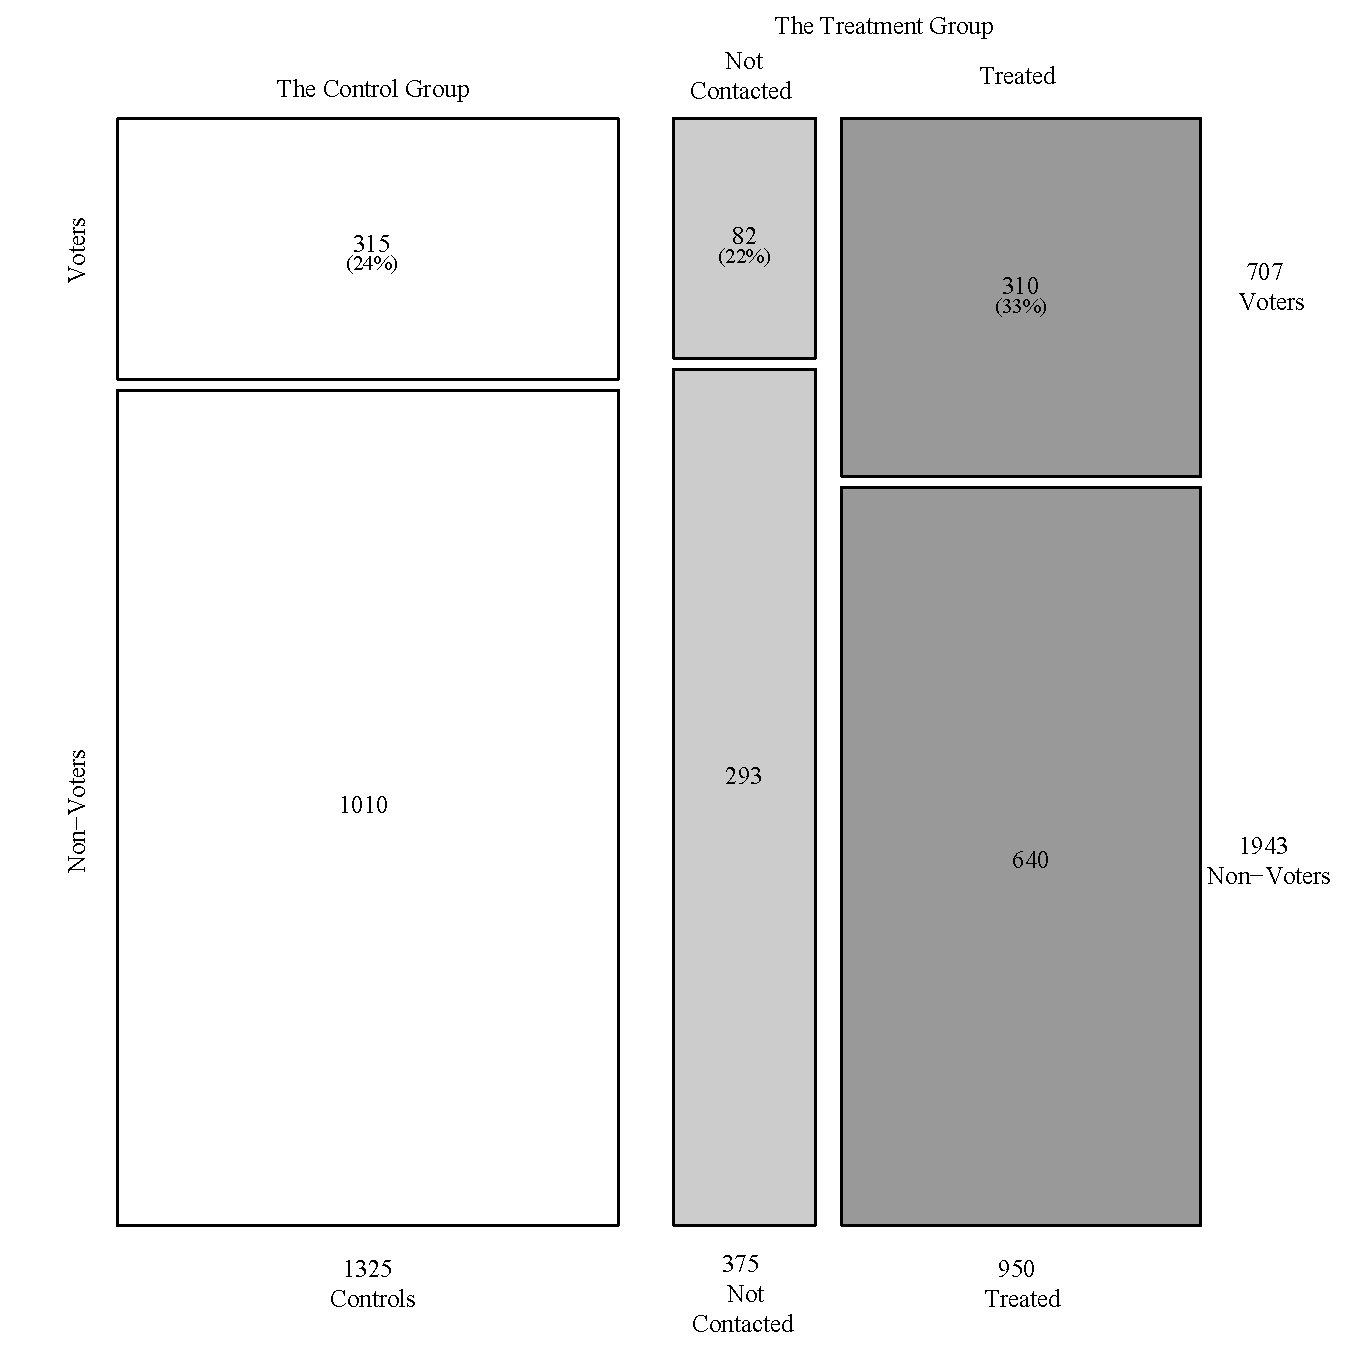
\includegraphics[height=.9\textheight]{images/ASdesign2edited}
\end{frame}
\note{As
  Angrist, Imbens and Rubin (1996) might have it, both groups are a
  blend of reachable and unreachable voters, although only for the Tx
  group are we able to distinguish the two; and it may well be that
  reachables and unreachables differ in terms of their voting
  behavior, even in the absence of any Tx.  The fact that
  non-contacted Tx group members voted less frequently than controls
  certainly suggests this.  For this reason few statisticians today
  would support Adams \& Smith's analytic strategy of simply comparing
  the treated to controls.}

\begin{frame}{The complier average causal effect via Bloom's(1984) method}

\begin{columns}
  \begin{Column}[.6\linewidth]    
    \begin{itemize}
  \item intention-to-treat effect ($\delta$) vs
    complier average causal effect (CACE; $\delta_{c}$).
 \item In terms of latent variable
   \{\underline{a}lways-taker/\underline{c}omplier/\underline{d}efier/\underline{n}ever-taker\},
   $\delta = p_{c}\delta_{c} + p_{a} \delta_{a} + p_{n} \delta_{n}
   + p_{d} \delta_{d}$.
    \end{itemize}
  \end{Column}
  \begin{Column}[.4\linewidth]
    \begin{tabular}{|r|c|c|}  \hline
      & \multicolumn{2}{c|}{$D_{z=1}$}\\
      $D_{z=0}$ & \multicolumn{1}{c}{1} &  \multicolumn{1}{c|}{0}\\ \hline
      1                &  a   &  d \\
      0                 & c   &  n \\ \hline
    \end{tabular}
  \end{Column}
\end{columns}
\vfill \pause

  \begin{itemize}[<+->]
  \item Assuming no effects for always-takers or never-takers
    (excludability), $\delta = p_{c} \delta_{c} + p_{d} \delta_{d} $.
  \item Assuming no defiers (monotonicity), $\delta = p_{c}
    \delta_{c}$. 
  \item Random assignment, non-interference $\Rightarrow$ both
    $\delta$ and $p_{c}$ are ACEs of assignment.
    \item Bloom's method is to estimate $\delta_{c}$ as the quotient
      of corresponding FACEs, $\hat\delta/\hat{p}_{c}$.
 \end{itemize}

\end{frame}
\itnote{
\item Couldn't make a cross-tab structured like the conceptual table at UR, b/c row and column position are jointly observed for no
  one. Instead, make progress w/ assumptions and estimation.
\item $\vdots$
\item State form of Bloom estimator}

\begin{frame} \frametitle{The Adams-Smith (1980) telephone GOTV
    experiment}
\framesubtitle{Contact rates by assignment condition}
  \begin{columns}
    \begin{column}{0.5\linewidth}
      \begin{tabular}{r@{\hspace{.5em}}rr} \hline
%  \multicolumn{2}{l}{Status} & $n$ \\
% \hline
\multicolumn{3}{l}{\underline{Telephone group}} \\
 & Contacted & 950 \\
 & No contact & 375 \\
 & all & 1325 \\ \hline
\multicolumn{3}{l}{\underline{Control group}} \\
 & Contacted & 0 \\
 & No contact & 1325 \\
 & all & 1325 \\  \hline
      \end{tabular}
    \end{column}
    \begin{column}{0.5\linewidth}
      \begin{tabular}{r@{\hspace{.5em}}rr} \hline
%  \multicolumn{2}{l}{Status} & $n$ \\
% \hline
\multicolumn{3}{l}{\underline{Telephone group}} \\
 & Voted &  392 \\
 & No vote &  \\
 & all & 1325 \\ \hline
\multicolumn{3}{l}{\underline{Control group}} \\
 & Voted &  315 \\
 & No vote &  \\
 & all & 1325 \\  \hline
      \end{tabular}
    \end{column}
  \end{columns}
\end{frame}


\begin{frame}{Exercises}
  \begin{columns}
    \begin{column}{0.4\linewidth}
      \begin{enumerate}[<+-\mynoteonly>]
      \item Estimate the ITT effect $\delta$.
      \item Identify the trap that was layed for
        you by this presentation of the data.  
      \item Estimate $p_{c}$. 
      \end{enumerate}
    \end{column}
    \begin{column}{0.6\linewidth}
      \igrphx{SalkVtable-observedonly.jpg}
    \end{column}
  \end{columns}
      \begin{enumerate}[<+-\mynoteonly>] \addtocounter{enumi}{3}
      \item Are there/may there be ``always-takers''?  
      \item Are there/may there be ``Never-takers''?
      \item Are there/may there be ``defiers''?
      \item Use Bloom's method to estimate the complier-average causal
        effect $\delta_{c}$.  How does your answer compare to the
        RCT's estimate of the ACE, $(41 -81) = -40$ cases per 100K
        innoculations?
      \end{enumerate}
\end{frame}

\end{document}

\begin{frame}{Average causal effects for samples of populations}
  
  \begin{itemize}
  \item Many writers assume 1,\ldots, n to be a sample from a
  broader population. Then notation $(Y_{T}, Y_{C})$ is appropriate
  (vs $(y_{T}, y_{C})$). 
  \item Random assignment ensures that $Z$ is independent of $Y_0$, $Y_1$.
  \item So under random assignment, $\mathrm{E}(Y_C|Z=0) =
  \mathrm{E}(Y_C)$;  $\mathrm{E}(Y_T|Z=1) = \mathrm{E}(Y_T)$.
  \item W/ simple, complete or paired rand. assmt, $\EE( \bar{Y}_{1}
  - \bar{Y}_{2}) = $ ACE. 
  \item Note that $Z$ is not generally independent of $Y=ZY_1 +
  (1-Z)Y_0$!
  \item Without random assignment, $\EE( \bar{Y}_{1}
  - \bar{Y}_{2}) = $ ACE may fail, even if the sample is perfectly
  representative of the population.
\item The ``samples'' from
  ``populations'' framing is sometimes invoked in order to apply apparati of conventional
  frequentist \& Bayesian inference.
  \end{itemize}
\end{frame}




